\documentclass{Head}
\begin{document}
\tableofcontents
\linenumbers
\section{Introduction}
Macromolecules are characterized by their long-chain structure, including molecular chain unit and conformation on angstrom scale, lamella on nanometer scale and spherulites on micron scale.
Nowadays, synchrotron radiation small angle X-ray scattering (SAXS) and wide angle X-ray diffraction (WAXD), as a non-destructive, highly statistically averaged structure analysis method, have been widely used in crystalline polymer research area.
For instance, study information on grains in crystalline polymer, micro-domains in blended polymers and the shape, size and distribution of cavities and cracks can be obtained by guinier scattering.
Study information on orientation, thickness and crystalline fraction of crystalline layer and the thickness of amorphous layer of the lamella can be obtained by long-period measurement.
\begin{figure}
    \centering
    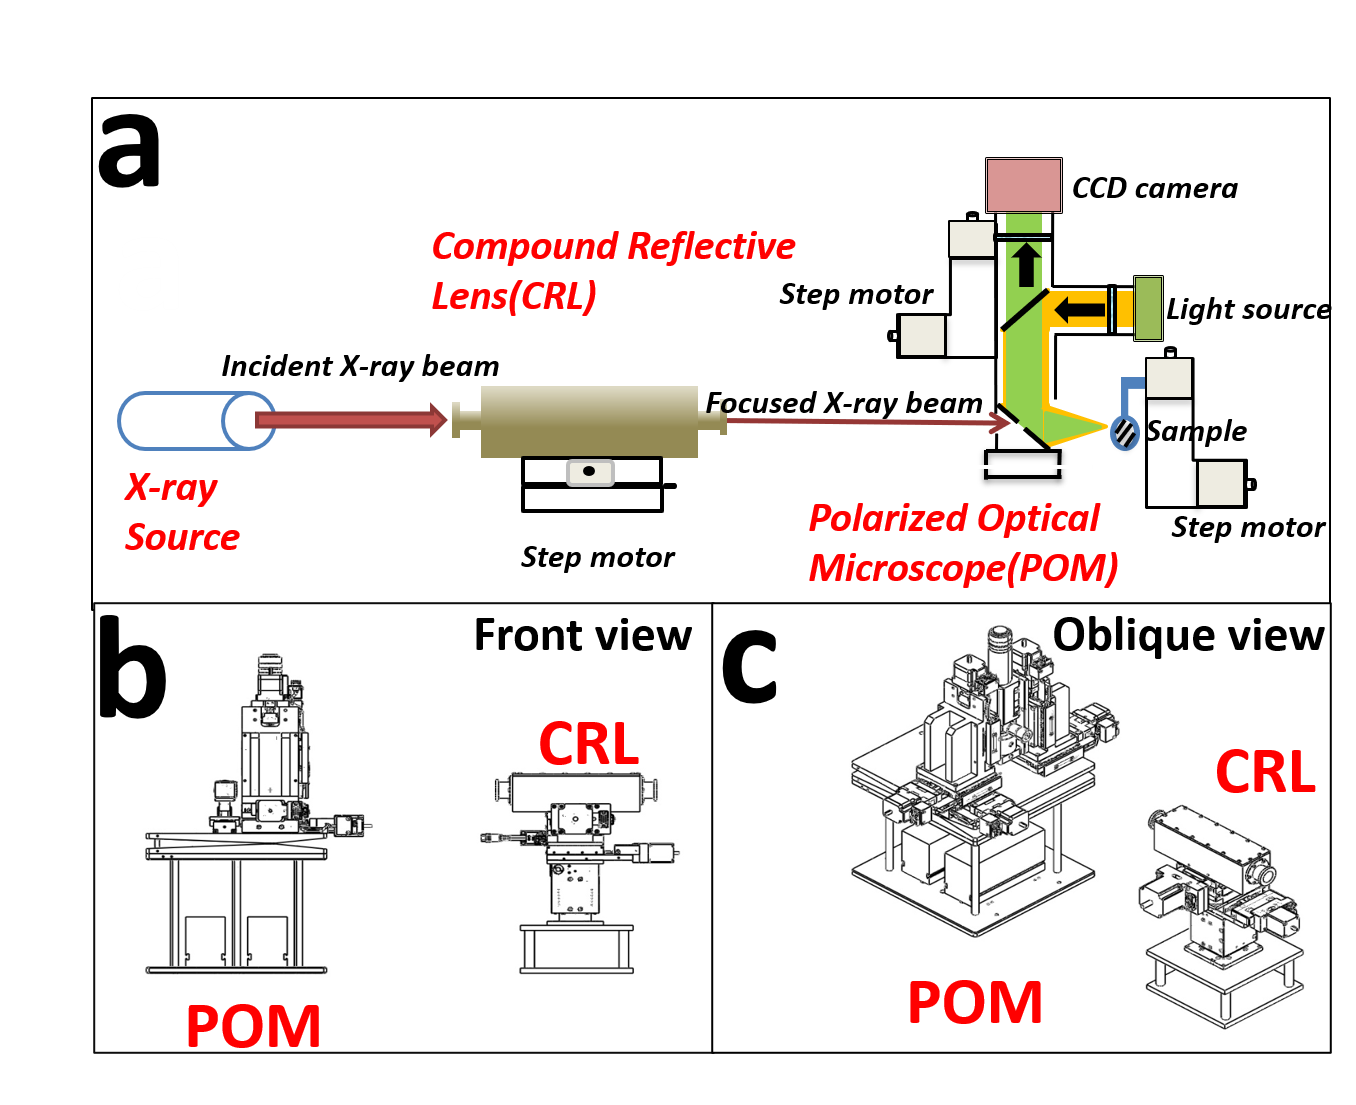
\includegraphics[scale=0.5]{Figures/Fig1WholeSystem.png}
    \caption{Whole system}
    \label{WholeSystem}
\end{figure}


In order to further study the internal structure of polymers, two new test condition are required.
Firstly, considering the size of polymer spherulites, an X-ray spot with a size of $5\mu m \cdot 5\mu m$ is needed.
A small spot provides sufficient spatial resolution when the structure of macromolecules are characterized by the SAXS method.
Secondly, In order to match the detection result with the real structure, confirming the real-time exact position of X-ray incident beam on polymer crystal is a critical measure.


To improve the spatial resolution of synchrotron radiation experiment, the world’s advanced synchrotron radiation light sources all use micro-focusing to focus the spot to the micron or even sub-micron level.
Representative beamline stations include DSEY-PETRA \uppercase\expandafter{\romannumeral3} P03, SSRF BL15U1.
However, limited by the distance between the sample and the detector, SAXS experiment can not be implemented on these stations.



The main components used for X-ray beam focusing are Kirkpatrick-Baez mirror, Fresnel zone plates, Capillary optical lens and Compound refractive lenses.
In synchrotron radiation area, Kirkpatrick-Baez mirror(K-B mirror) and Compound refractive lenses(CRLs) are more widely used.
The advantages of K-B mirror are aberration-free imaging on both horizontal and vertical planes, no dispersion, high energy, high reflectivity and low flux loss.
However, there are some disadvantages which should be considered.
K-B mirror micro-beam focusing needs to be achieved by adjusting the K-B two mirrors and multi-axis spatial attitude, including: the angle at which X-rays are incident on the mirrors, the vertical angle of the two mirrors, spatial parallelism of two vertical cylinders.
The deployment of K-B mirror changes the original optical path.
As a result, this off-axis device increases the complexity of installation of itself and other experimental equipment.
This is unfavorable for the entire micro-focusing experiment process.


Compound refractive lenses(CRL) are composed of a series of single lenses arranged in a linear array to achieve X-ray focusing in the energy range of 5-40 keV.
As shown in \autoref{CRL}, the most widely used CRL are parabolic compound refraction lenses.
The parabolic CRL has a parabolic surface that rotates around the axis of symmetry to form a parabola.
It can focus X-rays in two dimensions without causing aberrations in theory.
Compared to K-B mirror, CRL does not change the original optical path propagation direction, has good high temperature stability and easy cooling, simple and compact structure, easy to adjust, low requirements for lens' surface roughness, relatively insensitive to vibration and many other advantages.
The disadvantage of CRL is the low transmission efficiency.
Because the aperture of the diaphragm is small and the X-rays are absorbed when they penetrate the lens' material, the focused light intensity will drop by one to two orders of magnitude.
Despite this, the luminous flux can be maintained at $\mathrm{10^{10}\sim 10^{11} phs/s}$ after using CRL to focus the spot.
This flux is enough to study the structure of crystalline polymers.
\begin{figure}
    \centering
    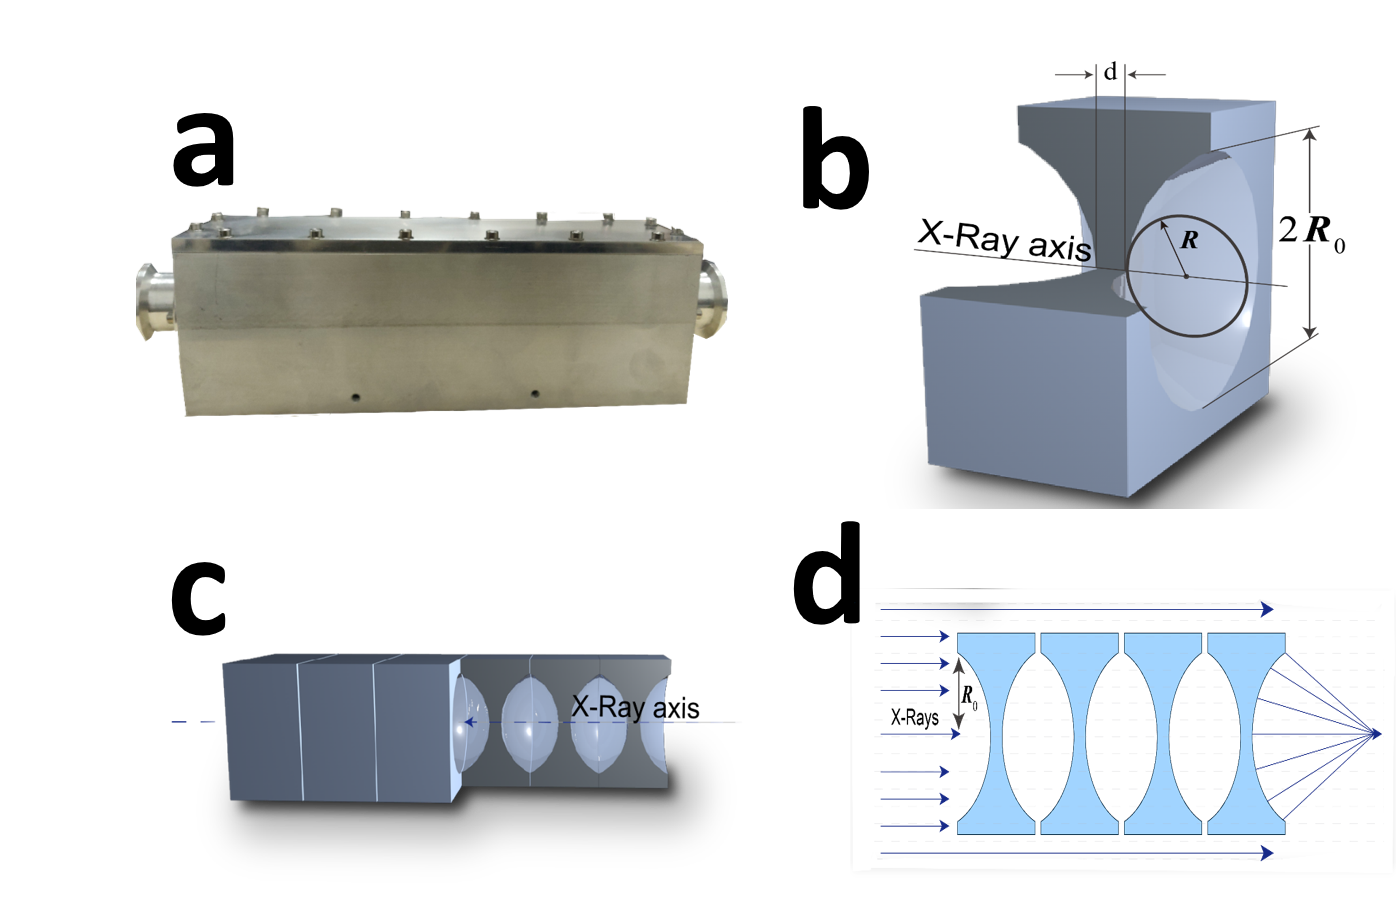
\includegraphics[scale=0.4]{Figures/Fig2CRL.png}
    \caption{Structure of Compound reflective lenses}
    \label{CRL}
\end{figure}


Polarized optical microscopy(POM) is widely used for studying polymer crystal morphology.
POM is a simple method to distinguish the change of growth direction of crystals in the film plane and to check whether there exists twisting of crystals\cite{RN37}.
\autoref{POM} is a schematic diagram of the disassembly of a POM.
When the polarized light generated by the polarizer and the analyzer enters the anisotropic polymer crystal, birefringence occurs, and the crystal contrast is obtained through the coherence of the polarized light.
Different crystal forms of polymers, such as spherulites, string crystals, stretched chain crystals, transverse crystals, etc., all have anisotropic optical properties, so their crystal morphology, size, number, etc. can be observed with a POM.
\begin{figure}
    \centering
    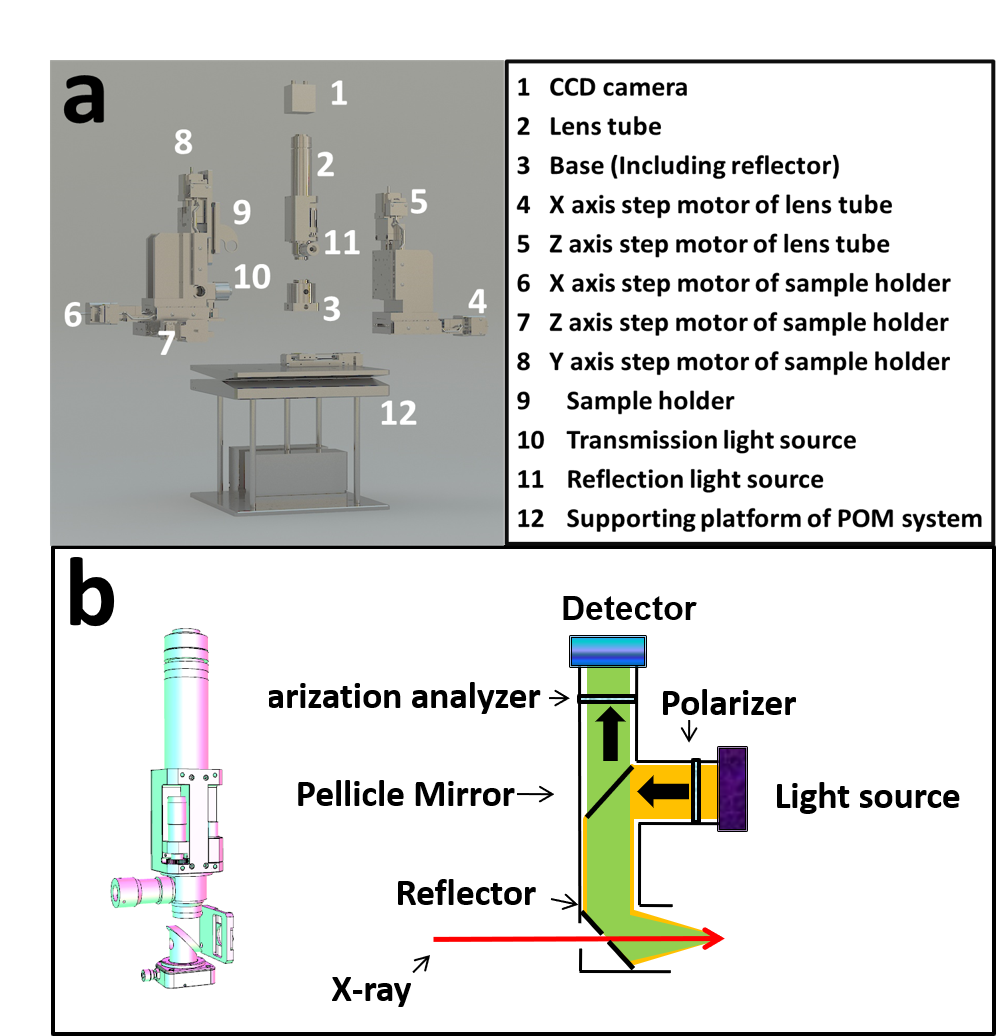
\includegraphics[scale=0.4]{Figures/Fig3POM.png}
    \caption{POM overall disassembly and lens cone disassembly.}
    \label{POM}
\end{figure}


In this passage, a combined device of micro-focus synchrotron radiation small-angle scattering and polarizing microscope is proposed.
A series of parameters of the device are adjusted, and the device is used to characterize the crystalline morphology and microstructure of related polymers.
\section{Experiment}
\subsection{Construction of stable light path}
\subsubsection{CRL parameter determination}
In order to obtain the designed X-ray microbeam, CRL's parameters need to be determined first.
The parameter mainly include material, geometric size and number of pieces.
Commonly used CRL is aluminum and beryllium.
According to the theory of atomic physics, materials with low atomic number have less absorption of X-rays. In this system, a beryllium CRL is chosen because the X-ray energy needs to be preserved as much as possible.



There are three common single mirrors.
The main geometric parameters of them are listed in \autoref{CRL parameters}.
First, CRL with a radius of 50 $\mathrm{\mu m}$ is selected to calculate the relevant parameters.
\begin{table}
    \centering
    \caption{Parameters of several common single lens}
    \begin{tabular}{ccc}
        \toprule
        Radius $R$/$\mathrm{\mu m}$ & Aperture 2$R_0$/$\mathrm{\mu m}$ & Area $\pi R_0^2$/$\mathrm{mm^{-2}}$ \\
        \midrule
        200                         & 881                              & 0.609                               \\
        100                         & 623                              & 0.305                               \\
        50                          & 440                              & 0.152                               \\
        \bottomrule
    \end{tabular}
    \label{CRL parameters}
\end{table}


Transmittance refers to the ratio of the light intensity after passing through the lens and the light intensity without passing through the lens.
It can be calculated by \autoref{transmission equation}\cite{Lengeler:ht2006}:
\begin{equation}
    T_p=\frac{\int_0^{2\pi}\mathrm{d}\theta\int_0^{R_0}e^{-\mu ND(r)}r\mathrm{d}r}{\int_0^{2\pi}\mathrm{d}\theta\int_0^{R_0}r\mathrm{d}r}=\frac{1-e^{-a}}{a}e^{-\mu Nd}
    \label{transmission equation}
\end{equation}
In \autoref{transmission equation}, $a=\mu N R_0^2/R$, $R$ and $R_o$ are given in \autoref{CRL parameters}, $N$ is the number of lens, $d$ is the minimum thickness of a single mirror.
For parabolic lenses, d can be calculated with the following equation:
\begin{equation}
    D(r)=d+2\times \frac{r^2}{2R}
    \label{width}
\end{equation}
The maximum processing thickness $D(r)$ of the CRL selected in this experiment is 2 mm.
Substituting $D(r)$ and $r=R_0$ into the \autoref{width}, the minimum d equals 1.032 mm.



According to the actual situation of beamline station shed size and pipeline layout, the image distance is about 400 mm and so is the focal length.
The focal length calculation formula under the approximate condition of thin lens is :
\begin{equation}
    f=R/2N\delta
\end{equation}
N is number of lenses, $\delta$ is real part of refractive index to 1 offset.
$\delta$ can be calculated by following equation\cite{als2011elements}:
\begin{equation}
    \delta=\frac{2\pi\rho r_o}{k^2}
\end{equation}
$\rho$ is electron number density, $r_o$ is the electronic classical radius.
For beryllium in 12KeV, $\delta$ is $2.36393\times 10^{-6}$.
When N is set to 30, the focal length is 352.5mm.
This value meets the requirements described above.
Substituting $N=30$ and $d=1.032$ into the \autoref{transmission equation}, $T_p$ equals 0.327.


The flux of photons after passing through the lenses can be calculated by the following equation:
\begin{equation}
    I=i\times T_p \times R
    \label{intensity}
\end{equation}
$i$ is the flux of incident X-ray.
In BL19U2, under 220 mA current intensity, $i=2.5\times 10^{12}$ photons/s, $R$ is defined as the photon acceptance rate and equals 0.0598.
Substituting these values into the \autoref{intensity}, $I$ equals $4.89\times 10^{10}$ photons/s. This value is enough to study the structure of crystalline polymers.


For lens with a radius of 100$\mu$m and 200$\mu$m, after the same calculation, N is 60 and 120.
Although a lens with a larger radius of curvature can be used to obtain a slightly larger flux, the number of lenses required is greatly increased.
Comprehensive consideration, using 30 lenses with a radius of 50 $\mu$m is the best choice.
\subsubsection{Reduce beam jitter}
Due to the thermal load caused by the high-power beam to the monochromator crystal and the vibration of the monochromator crystal caused by the liquid nitrogen cooling system of the monochromator, the current spot of the BL19U2 is jittered by about 10\%, which will affect the strength stability of X-ray micro beam.


A processing software is compiled which integrates light intensity position data collection, data processing (calculation of beam center), data smoothing and filtering, PID control algorithm and control interface.
Advanced FPGA technology is applied to design and implement a fuzzy adaptive PID controller.
Beam position which is collected by the PID control loop in real time is compared with the set value.
Then the comparison error is sent to the PID controller to calculate the control value through the PID control algorithm.
Subsequently, the comparison error is input to the actuator of the monochromator pizeo to adjust the pizeo angle of the second crystal in real time, realize the constant feedback system of the beam center position and the constant light intensity feedback system.
Finally, it is realized that the closed-loop control of the beam position and suppress low the beam drift of the frequency band to realize the stabilization of the BL19U2.
Thus, the impact of beam jitter on the intensity of the focused beam is reduced.
\subsection{Construction of the combined system}

\autoref{WholeSystem} is the schematic diagram of the structure of synchrotron radiation X-ray micro-focusing polarized microscopy system.
The combined system includes a micro-focusing component and an in situ polarized light microscope system.
After the incident X-ray is focused by the CRL, it will pass through the light hole on the lower side of the POM and the sample, then the scattered signal will be received by the detector.
The on-site construction diagram of the system is shown in \autoref{sitemap}.
\begin{figure}
    \centering
    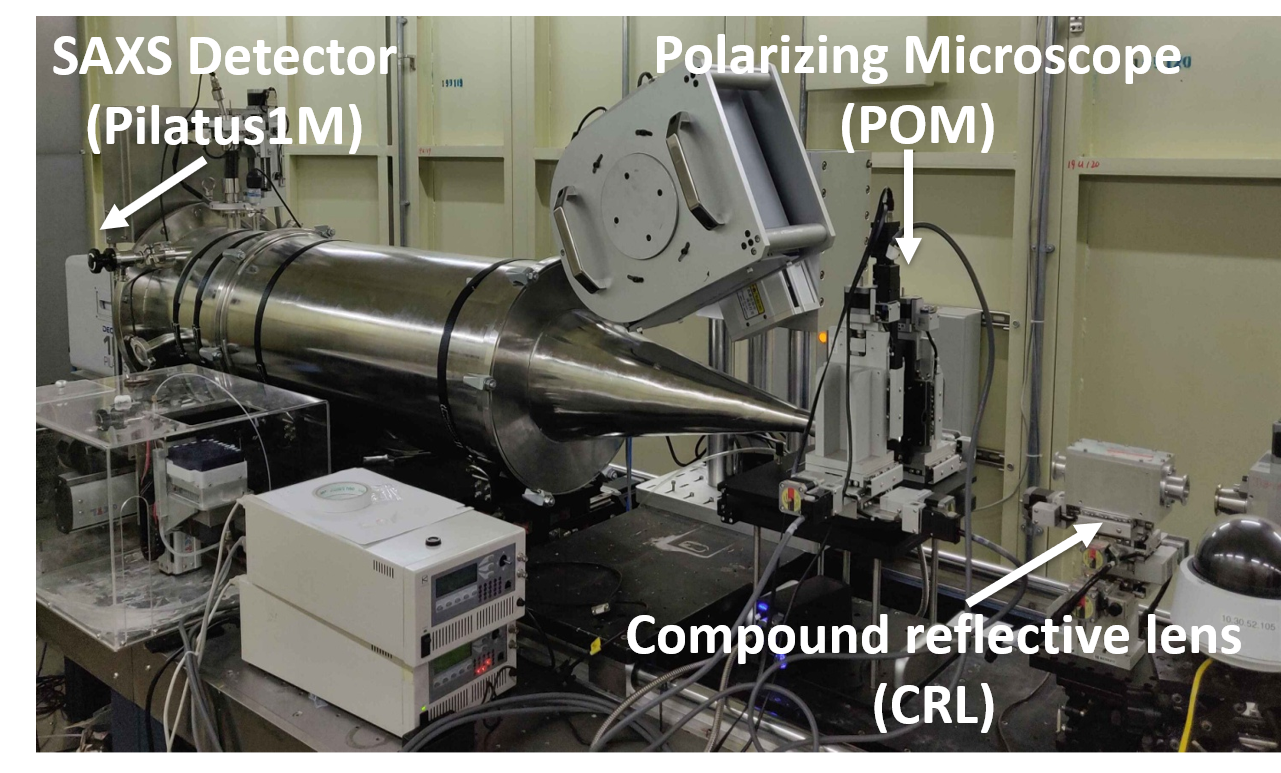
\includegraphics[scale=0.5]{Figures/Fig4SiteMap.png}
    \caption{Site map of the combined system.}
    \label{sitemap}
\end{figure}

As shown in \autoref{WholeSystem}, the CRL is mounted on a motorized platform. Including three-dimensional translational electric platform (x, y, z three directions), one-dimensional swing stage (P angle) and one-dimensional rotating platform (R angle). The posture of CRL can be adjusted in five spatial dimensions.


The structure of POM used in the system is shown in \autoref{POM}.
As shown in \autoref{POM}b, the optical system of POM mainly consists of the following parts: a polarizer and analyzer that use ordinary white light sources to generate polarized light; a half mirror located in the middle of the lens barrel; A flat mirror located at the bottom of the lens barrel. The detector at the top is used to collect images. In this system, the detector selects a Charge-coupled device(CCD) camera.


As shown in \autoref{POM}a, the in situ POM system is also installed on a motorized support platform.
A stepping motor (4$\sim$5) installed on the side of the lens body realizes the translational adjustment of the lens barrel in two dimensions.
Similarly, the stepping motor (6$\sim$8) on the side of the sample holder realizes its translational adjustment in three dimensions.
The supporting platform (12) can be further divided into three layers: the uppermost layer is a one-dimensional swing stage and a rotating table, the middle layer is a two-dimensional (horizontal) translational electric platform, and the lowest layer is a three-dimensional translational electric platform.
Through the adjustment devices in all the above dimensions, The five spatial dimensions of the entire optical system can be adjusted.
\subsection{Determination of spot parameters}
Once the combined system is installed in beamline, the beam can be adjusted.
The main purpose of beam adjustment is threefold: first, to ensure the connectivity of the integrated optical path, to ensure that X-rays can pass through the system correctly.
A series of elements on the fixed light path of the beamline are used to adjust the primary light spot, and then the light path is adjusted using the POM and CRL spatial dimensions.
The current value of the ionization chamber can determine whether there is enough X-ray flux to irradiate the sample.
The second purpose is to verify whether the CRL is accepted to focus the primary spot to a sufficiently small spot size.
Only when the size is basically in line with the theoretical value to achieve a sufficiently small spatial resolution, can the microstructure of the research system be characterized; the third is to adjust the position of the light spot to the center of the field of view, while adjusting the angle of the plane mirror to make the The polarized light that reaches the sample after being reflected twice by the half mirror and the plane mirror is focused on the X-ray at this point in the sample.
The detection point of the sample is located in the center of the field of view, and the detection position will not shift even if the magnification of the polarizing microscope is changed.
In order to achieve the latter two purposes, we need to observe the spot in real time under POM.
For this reason, we install a cesium iodide crystal on the sample stage. Cesium iodide crystal has the characteristic of emitting fluorescence under X-rays, so it is also called scintillation crystal. In this system, the X-ray spot position is calibrated by the fluorescence spectrum generated by cesium iodide under POM.
\begin{figure}
    \centering
    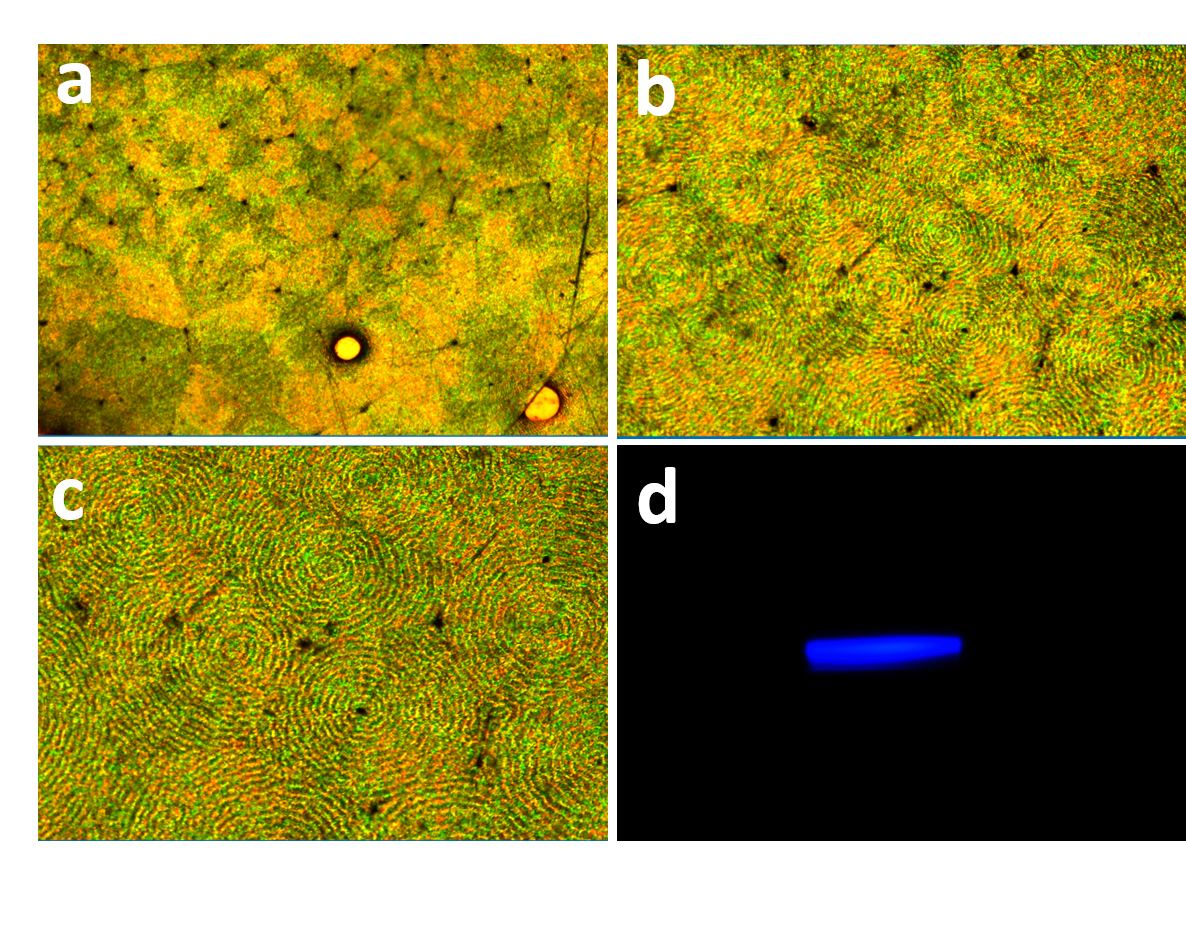
\includegraphics[scale=0.5]{Figures/Fig5CommissionPOMOnSite.png}
    \caption{Result of commissioning POM on site}
    \label{pictures}
\end{figure}


The step motors used in this system are all produced by Kohzu Corporation.
The positioning accuracy can reach 1um, which is enough for precise spatial position adjustment.
Adjust the CRL posture so that the incident X-ray can pass through the lenses correctly and be focused.
Then adjust the y-direction motor of the POM sample stage, so that the scintillation crystal is correctly focused and imaged in the field of view of the polarizing microscope.
Finally, adjust the x and z direction motors to move the center of the field of view to the fluorescent spot.
In the PC imaging software, a cross ruler will be displayed to assist in positioning.



The theoretical focus size of the focus spot is about 5um 5um.
In order to verify the difference between the actual adjustment and the theoretical calculation, two methods are usually used.
As shown in Figures 6a and 6b, the first is to visually observe through imaging software and use a ruler to make rough measurements.
This method is relatively intuitive and fast, but the accuracy is insufficient.
The second method is to use ionization chamber current data for fitting.
According to related theories, FWHM of the first derivative of ionization chamber current to displacement can refer to the spot size.
The representative fitting results of this system are shown in \autoref{fitting}c, As shown in \autoref{fitting}d, Gaussian fitting is performed on the original curve, and the FWHM of the fitted peak is calculated to be 5.43$\mu$m$\times$6.52$\mu$m.
This value can represent the effective size of the light spot, and this value basically achieves the expected effect.
\begin{figure}
    \centering
    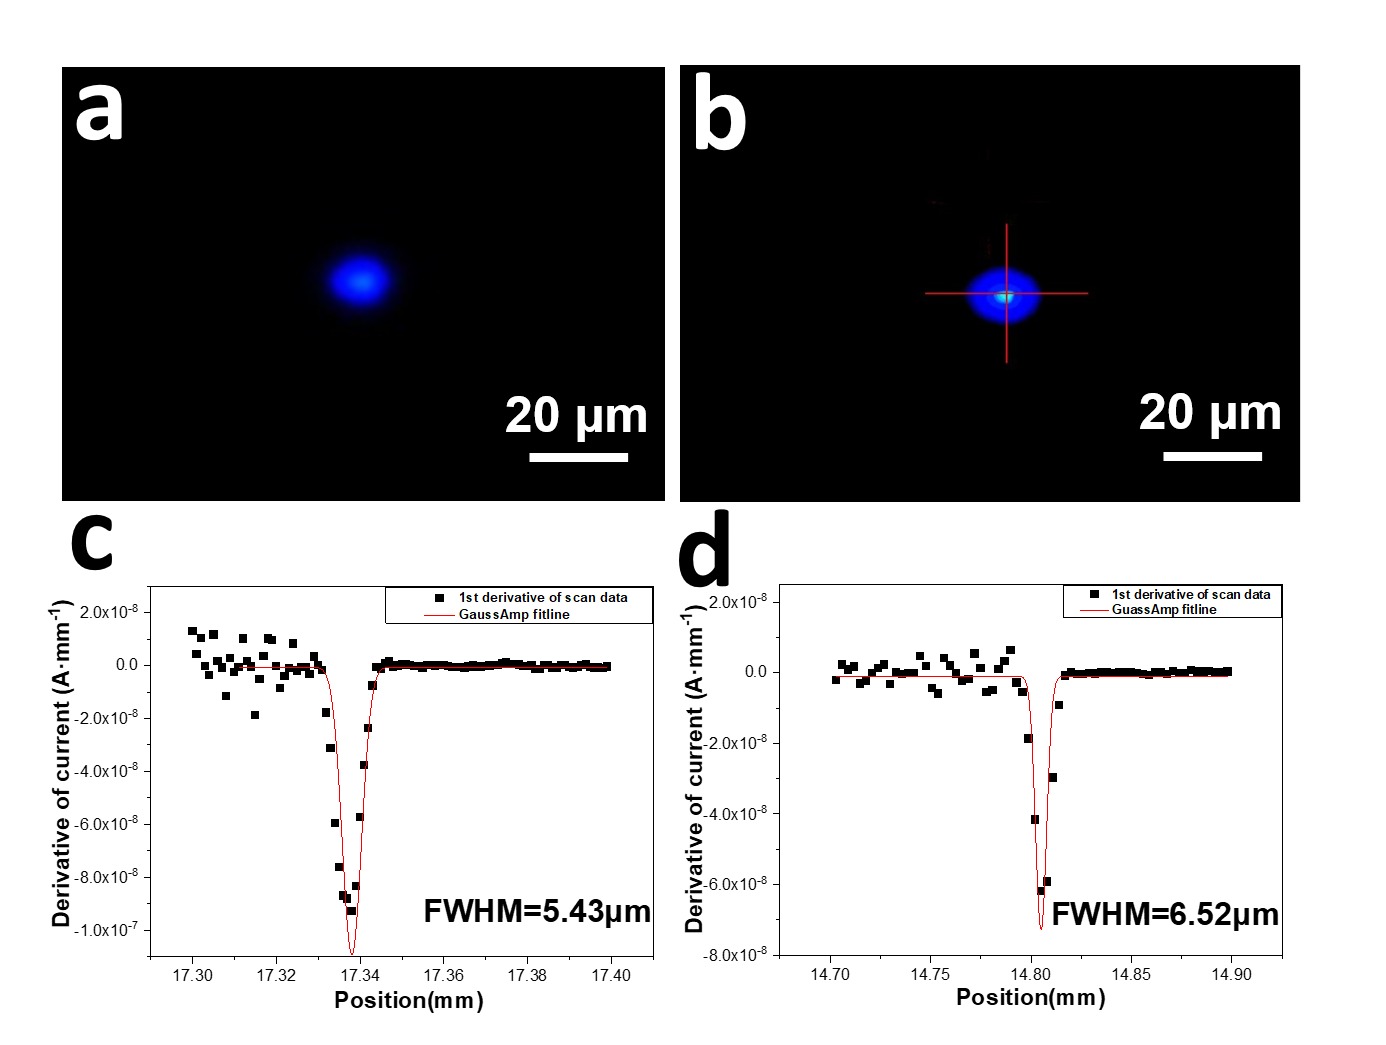
\includegraphics[scale=0.5]{Figures/Fig6CRLmicrofocus.png}
    \caption{Result of CRL micro-focus (facula and flux)}
    \label{fitting}
\end{figure}
\subsection{Collection of micro-focus X-ray scattering data}
After adjusting the size and position of the light spot, it can be used to characterize the micro-domain structure of related polymer crystals.
First, determine the position that needs to be characterized under the POM, and then use the motor installed on the platform to remove the visible light source. Pass in synchrotron X-rays to collect scattered signals.
At the SSRF-BL19U2 line station, X-rays with an energy of 12keV are often used, and the distance between the sample and the detector is 2700mm.
The scattering signal is collected by Pilatus1M detector (981*1043pixel, with a pixel size of 172um*172um).


\section{Application}
In order to verify the feasibility of the entire combined system, the spherulites with annulus and fibers with a sheath-core structure are used as research examples.
Micro-focused X-ray spot is used for micro-area resolution, and the scattering information of small structures that cannot be obtained by ordinary small-angle scattering experiments can be obtained.
\subsection{Microstructure of ringed sperulites}
Spherulites are the most common morphological structure of polymer materials, and they also play a vital role in the physical, chemical and mechanical properties of polymer materials. Its multi-level structure is complicated, and many basic scientific issues related to its structure need to be further explored.
At present, in the study of the microstructure of zonal spherulites, there are several scientific problems that need to be explained urgently. The first problem is the correlation between the growth axis of the polymer ring-belt spherulites and the torsion chirality of the lamellae.
One theory is that the growth axis affects the chirality of the lamella torsion by changing the pressure distribution on the lamella plane.
micro-focus X-ray can be used to determine the growth axis of each region and the tilt torsion behavior of the mapping crystal plane along the growth axis, revealing the correlation between the crystal growth axis and the lamella torsion chirality. It can provide a scientific basis for clarifying the transfer behavior of chirality between the multi-level structure of polymer spherulites.
The second problem is the cross-nucleation of polymer spherulites during the crystallization.
Through micro-focus X-ray, the crystalline transformation information at the front of spherulite growth are monitored in situ, including crystal plane, orientation, whether there is a transition (gradient) zone to reveal the cross-nucleation mechanism in polymer crystals, and clarify multiple crystal types the correlation and the similarities and differences between polymer cross nucleation and traditional cross nucleation of small molecule.
\begin{figure}
    \centering
    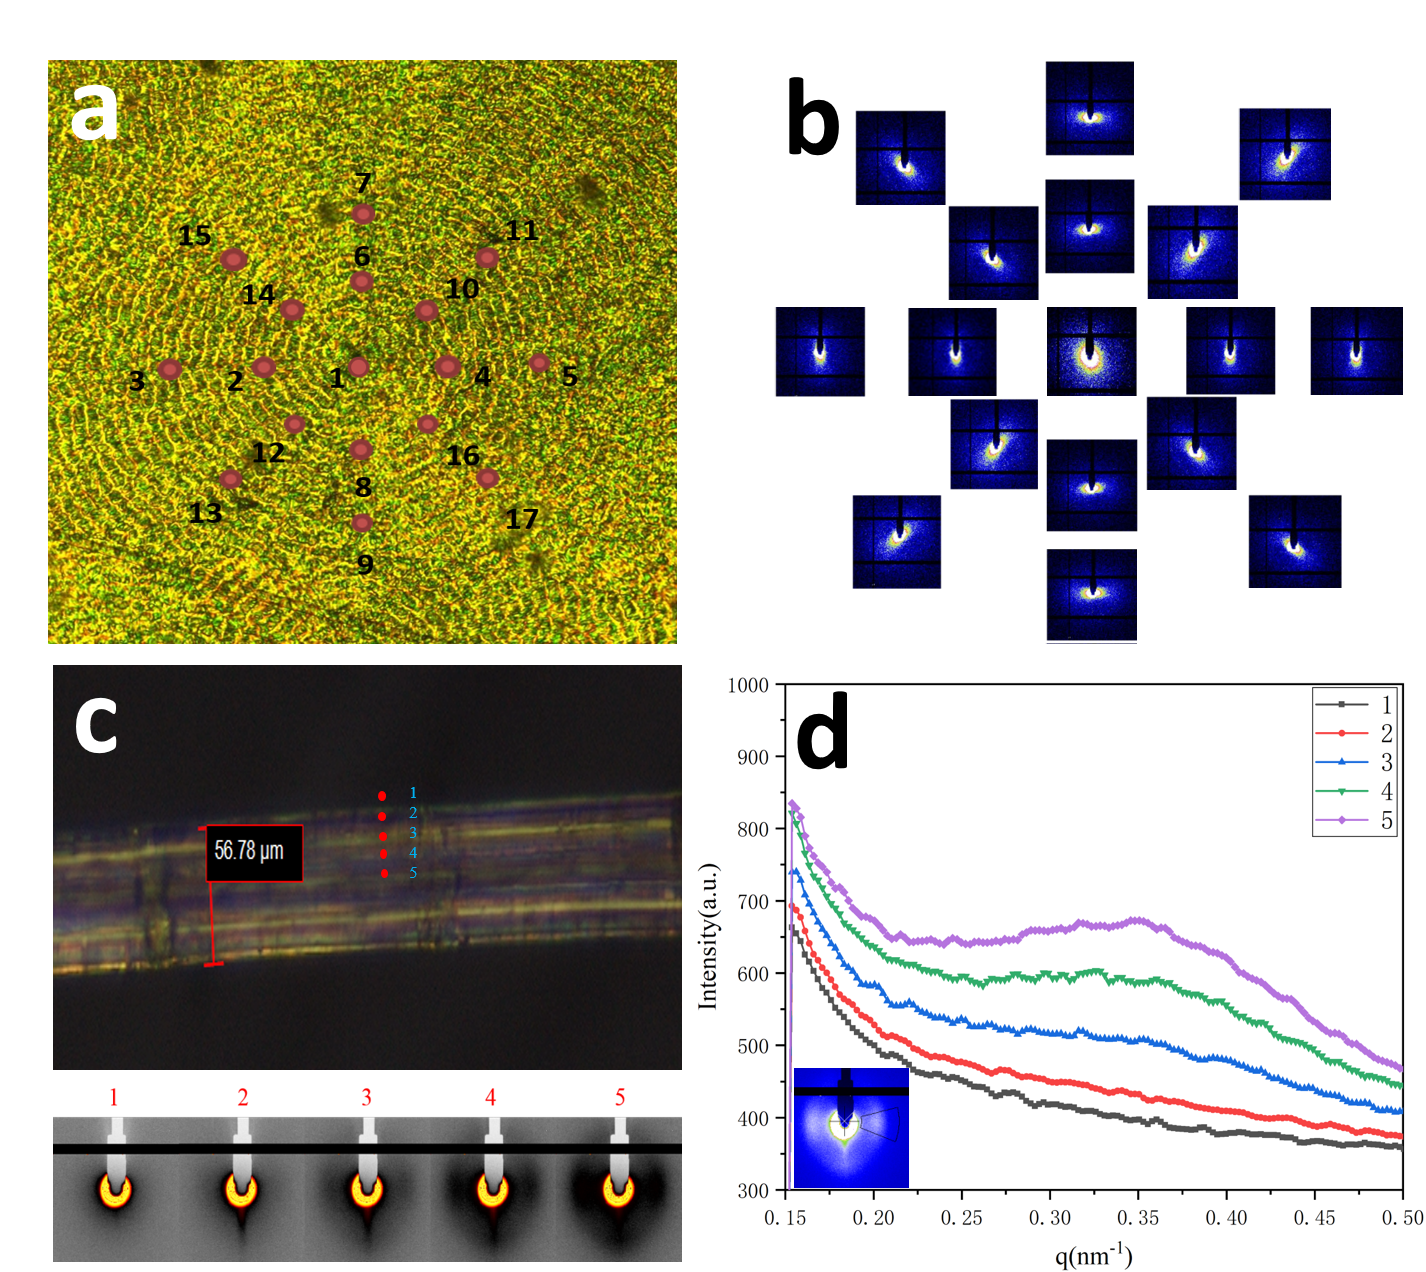
\includegraphics[scale=0.5]{Figures/Fig7AppliedResearch.png}
    \caption{The application sample of the system}
\end{figure}


We chose banded spherulites as a sample to verify the usability of the micro-focusing polarizing microscope system.
Microbeam X-ray scans are especially informative.
\subsection{The skin and core structure of the fiber}
\section{Conclusion}
\bibliography{reference.bib}
\end{document}